% Chapter 3 -- Scattering by a central potential (Goldstein Sec. 3.10).
%
% Reference convention: Goldstein, Poole & Safko, "Classical Mechanics,"
% 3rd ed., Ch. 3, Sec. 3.10 "The Scattering Problem in a Central Force,"
% adopted for terminology and equation style. Symbols follow this
% document's own declarations below, which govern wherever they differ
% from Goldstein's (per the scope note in goldsteinnotes.sty).

\documentclass[11pt]{article}
\usepackage{goldsteinnotes}
\usepackage{tikz}
\usepackage{cancel}
\usepackage{sectsty}
\usetikzlibrary{arrows.meta,calc}

\allsectionsfont{\boldmath}

% Numbering carries the chapter, so sections and equations read 3.n.
\renewcommand{\thesection}{3.\arabic{section}}
\renewcommand{\theequation}{3.\arabic{equation}}
\renewcommand{\thefigure}{3.\arabic{figure}}

% --- symbols fixed for THIS document (see the scope note in goldsteinnotes.sty)
% m       : mass of the incident particle
% \ell    : conserved angular momentum
% s       : impact parameter (Goldstein's own symbol; kept, not Taylor's b)
% \theta  : scattering angle (final, measured quantity)
% \psi    : apsidal angle
% \tilde\theta, \tilde\theta' : running orbit angle and its integration
%           constant in the Coulomb orbit equation, tilded to distinguish
%           them from the scattering angle \theta above
% \varepsilon : orbit eccentricity
% \sigma_T    : total cross section (kept with the subscript, not bare \sigma)
\renewcommand{\vect}[1]{\vec{#1}}
\renewcommand{\unit}[1]{\hat{#1}}

\newcommand{\Om}{\Omega}
\newcommand{\half}[1]{\tfrac{#1}{2}}

\title{Scattering by a Central Potential}
\author{}
\date{}

\begin{document}
\maketitle
\vspace{-2.5em}

\section{Kinematics and the Differential Cross Section}

\begin{align}
\text{Incident energy:}\quad & E = \frac{m}{2}v_0^2, &
\text{Incident velocity:}\quad & v_0 = \sqrt{2E/m}, \\
\text{Angular momentum:}\quad & \ell = s\,m\,v_0 = s\sqrt{2mE}, &
& s = \frac{\ell}{\sqrt{2mE}}.
\end{align}

The volume element in spherical coordinates is
\begin{equation}
d^3r = r^2\,dr\,\underbrace{d\varphi\,\sin\theta\,d\theta}_{\displaystyle d\Om},
\end{equation}
and since the azimuthal angle $\varphi$ is irrelevant by symmetry, integrating
it out gives the solid angle subtended by a ring of scattering angles between
$\theta$ and $\theta+d\theta$:
\begin{equation}
d\Om = 2\pi\sin\theta\,d\theta.
\end{equation}
Because the impact parameter and the scattering angle are in one-to-one
correspondence, $s\leftrightarrow\theta$, the deflection is fully controlled by
the function $s(\theta,E)$ (Fig.~\ref{fig:ring}).

\begin{figure}[htbp]
\centering
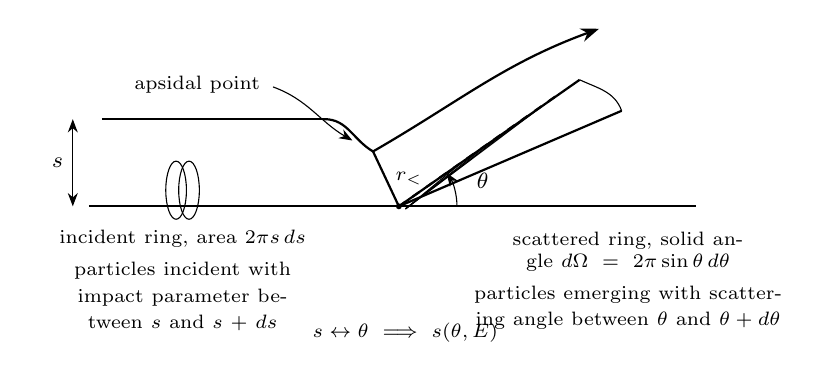
\begin{tikzpicture}[scale=0.82,>=Stealth,every node/.style={font=\footnotesize}]
  % main axis
  \draw[thick] (-4.8,0) -- (4.6,0);
  \coordinate (O) at (0,0);
  \fill (O) circle (1.3pt);
  % incident beam at height s, bending through the apsidal point
  \coordinate (P) at (-0.4,0.85);
  \draw[thick] (-4.6,1.35) -- (-1.15,1.35);
  \draw[thick] (-1.15,1.35) to[out=0,in=150] (P);
  \draw[thick,->] (P) to[out=30,in=200] (3.1,2.75);
  \draw[thick] (P) -- (O);
  \node[right] at ($(P)!0.5!(O)$) {\scriptsize $r_{<}$};
  \draw[->] (-1.95,1.85) to[out=-20,in=150] (-0.72,1.02);
  \node[left] at (-2.0,1.88) {\scriptsize apsidal point};
  % impact parameter s
  \draw[<->] (-5.05,0) -- (-5.05,1.35);
  \node[left] at (-5.05,0.68) {$s$};
  % incident ring icon
  \draw (-3.45,0.25) ellipse (0.16 and 0.45);
  \draw (-3.25,0.25) ellipse (0.16 and 0.45);
  % theta angle at O, reference ray parallel to outgoing asymptote
  \draw[thick,dashed] (O) -- (2.45,1.72);
  \draw[->] (0.9,0) arc (0:35:0.9);
  \node at (1.3,0.40) {$\theta$};
  % scattered ring (cone between theta and theta+dtheta)
  \draw[thick] (O) -- (2.8,1.96);
  \draw[thick] (O) -- (3.45,1.48);
  \draw (2.8,1.96) to[out=-25,in=110] (3.45,1.48);
  \foreach \t in {0.35,0.5,0.65,0.8} {
    \draw (O)+({\t*2.8},{\t*1.96}) -- +({0.11*0.93},{-0.11*0.36});
  }
  % captions, well clear of the diagram and of each other
  \node[align=center,text width=3.7cm] at (-3.35,-1.15)
    {\scriptsize incident ring, area $2\pi s\,ds$\\[2pt]
     \scriptsize particles incident with impact parameter between $s$ and $s+ds$};
  \node[align=center,text width=4.0cm] at (3.55,-1.15)
    {\scriptsize scattered ring, solid angle $d\Om=2\pi\sin\theta\,d\theta$\\[2pt]
     \scriptsize particles emerging with scattering angle between $\theta$ and $\theta+d\theta$};
  \node at (0.1,-1.95) {\scriptsize $s\leftrightarrow\theta \ \Longrightarrow\ s(\theta,E)$};
\end{tikzpicture}
\caption{Particles incident in the ring of area $2\pi s\,ds$ emerge into the
ring of scattering angles between $\theta$ and $\theta+d\theta$; $r_{<}$ is the
distance of closest approach, reached at the apsidal point. The azimuthal
angle is irrelevant by symmetry.}
\label{fig:ring}
\end{figure}

\subsection{Incident Intensity and the Differential Cross Section}

\begin{equation}
I = \frac{\#\ \text{particles incident per unit time}}
         {\text{incident beam cross-section area}},
\end{equation}
\begin{equation}
\sigma(\Om)\,d\Om =
\frac{\#\ \text{particles scattered into }d\Om\text{ per unit time}}
     {\text{incident intensity}}.
\end{equation}

\begin{align}
I\,(2\pi s)\,\lvert ds\rvert
  &= \#\ \text{particles going through the ring between } s \text{ and } s+ds\notag\\
  &= \#\ \text{particles emerging with angle between } \theta \text{ and } \theta+d\theta\notag\\
  &= I\,\sigma(\theta)\,2\pi\sin\theta\,\lvert d\theta\rvert.
\end{align}

Therefore
\begin{equation}
\boxeq{\ \sigma(\theta) = \frac{s}{\sin\theta}\left\lvert \dd{s}{\theta}\right\rvert\ }
\label{eq:sigma-def}
\end{equation}
and the total cross section is defined by
\begin{equation}
\boxeq{\ \sigma_T = \int d\Om\ \sigma(\Om)\ }.
\label{eq:sigmaT-def}
\end{equation}

\section{General Relation between Impact Parameter and Scattering Angle}

\begin{figure}[htbp]
\centering
\begin{minipage}[b]{0.47\textwidth}
\centering
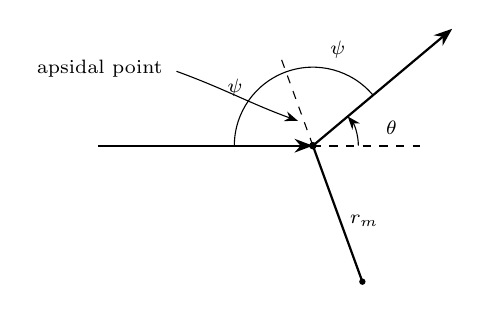
\begin{tikzpicture}[scale=1.05,>=Stealth,every node/.style={font=\footnotesize}]
  \coordinate (V) at (0,0);
  \fill (V) circle (1.3pt);
  \draw[thick,->] (-2.6,0) -- (V);
  \draw[thick,dashed] (V) -- (1.3,0);
  \draw[thick,->] (V) -- (40:2.2);
  \draw[dashed] (V) -- (110:1.15);
  \coordinate (C) at (290:1.75);
  \fill (C) circle (1.1pt);
  \draw[thick] (V) -- (C);
  \node[right] at ($(V)!0.55!(C)$) {\scriptsize $r_m$};
  \draw[->] (0.55,0) arc (0:40:0.55);
  \node at (0.95,0.22) {\scriptsize $\theta$};
  \draw (40:0.95) arc (40:110:0.95);
  \node at (0.30,1.16) {\scriptsize $\psi$};
  \draw (110:0.95) arc (110:180:0.95);
  \node at (-0.94,0.70) {\scriptsize $\psi$};
  \draw[->] (-1.65,0.90) to[out=-20,in=160] (-0.18,0.30);
  \node[left] at (-1.7,0.93) {\scriptsize apsidal point};
\end{tikzpicture}\\[2pt]
{\small Repulsive case}
\end{minipage}\hfill
\begin{minipage}[b]{0.47\textwidth}
\centering
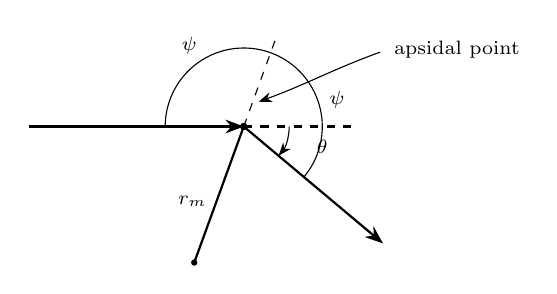
\begin{tikzpicture}[scale=1.05,>=Stealth,every node/.style={font=\footnotesize}]
  \coordinate (V) at (0,0);
  \fill (V) circle (1.3pt);
  \draw[thick,->] (-2.6,0) -- (V);
  \draw[thick,dashed] (V) -- (1.3,0);
  \draw[thick,->] (V) -- (-40:2.2);
  \draw[dashed] (V) -- (70:1.15);
  \coordinate (C) at (250:1.75);
  \fill (C) circle (1.1pt);
  \draw[thick] (V) -- (C);
  \node[left] at ($(V)!0.55!(C)$) {\scriptsize $r_m$};
  \draw[->] (0.55,0) arc (0:-40:0.55);
  \node at (0.95,-0.24) {\scriptsize $\theta$};
  \draw (-40:0.95) arc (-40:70:0.95);
  \node at (1.13,0.32) {\scriptsize $\psi$};
  \draw (70:0.95) arc (70:180:0.95);
  \node at (-0.66,0.98) {\scriptsize $\psi$};
  \draw[->] (1.65,0.90) to[out=200,in=20] (0.18,0.30);
  \node[right] at (1.7,0.93) {\scriptsize apsidal point};
\end{tikzpicture}\\[2pt]
{\small Attractive case}
\end{minipage}
\caption{The apsidal angle $\psi$ and the scattering angle $\theta$ in the
repulsive and attractive cases; $r_m$ is the distance of closest approach.}
\label{fig:cases}
\end{figure}

\begin{center}
\begin{tabular}{@{}l@{\qquad}l@{}}
\textsc{Repulsive case} & \textsc{Attractive case}\\[4pt]
$\pi = \theta + 2\psi$ & $\pi = 2\psi - \theta$\\[2pt]
$\theta = \pi - 2\psi$ & $\theta = 2\psi - \pi$\\[2pt]
$\psi = \dfrac{\pi-\theta}{2}$ & $\psi = \dfrac{\pi+\theta}{2}$
\end{tabular}
\end{center}

In all cases:
\begin{equation}
\boxeq{\ \theta = \lvert\, \pi - 2\psi\, \rvert\ }
\label{eq:allcases}
\end{equation}

\subsection{Computing \texorpdfstring{$s(\theta,E)$}{s(theta,E)}: the Universal Method}

\begin{equation}
E = \frac{m}{2}\dot r^{2} + V(r) + \frac{\ell^{2}}{2mr^{2}},
\qquad
\dot r = \left[\frac{2}{m}\left(E - V(r) - \frac{\ell^{2}}{2mr^{2}}\right)\right]^{1/2},
\qquad
\dot r = \dd{r}{t} \;\Rightarrow\; dt = \frac{dr}{\dot r}.
\end{equation}

\begin{align}
\ell = m r^{2}\dot\theta \;\Rightarrow\;
\dd{\theta}{t} = \dot\theta = \frac{\ell}{mr^{2}}
\;\Rightarrow\;
d\theta &= \dot\theta\,dt = \frac{\ell}{mr^{2}}\,dt
 = \frac{\ell}{mr^{2}}\,
   \frac{dr}{\left[\frac{2}{m}\left(E-V(r)-\frac{\ell^{2}}{2mr^{2}}\right)\right]^{1/2}}\notag\\[4pt]
 &= \underbrace{\frac{\ell}{m}\sqrt{\frac{m}{2E}}}_{\displaystyle =\;\frac{\ell}{\sqrt{2mE}}\;=\;s}\;
    \frac{r^{-2}\,dr}{\left[1 - \dfrac{V(r)}{E}
      - \underbrace{\dfrac{\ell^{2}}{2mE}}_{\displaystyle =\;s^{2}}\dfrac{1}{r^{2}}\right]^{1/2}}.
\end{align}

Integrating from the apsidal point out to infinity gives the apsidal angle
$\psi$;\footnote{The integrand of the $r$-integral below carries $V(r)$
rather than $V(r)/E$, while the boxed result on the same line correctly
carries $V(1/u)/E$; the inconsistency is retained rather than normalized.} the substitution
$u=1/r$ is then made.\footnote{Written as $u=1/r$, $du=r^{-2}dr$; the missing
sign on $du$ is absorbed by the interchange of the limits of integration.}

\begin{gather}
\psi = \int_{0}^{\psi}d\psi = \int_{\theta_{m}}^{\pi}d\theta
     = \int_{r_{m}}^{\infty} \frac{s\,r^{-2}\,dr}
       {\bigl[1 - V(r) - s^{2}/r^{2}\bigr]^{1/2}}\,,
\qquad
u = \frac{1}{r},\quad du = r^{-2}\,dr,\quad u_{m} = \frac{1}{r_{m}}\notag\\[6pt]
\Longrightarrow\quad
\boxeq{\ \theta(s) = \left\lvert\, \pi - 2\int_{0}^{u_{m}}
  \frac{s\,du}{\left[1 - \dfrac{V(1/u)}{E} - s^{2}u^{2}\right]^{1/2}} \,\right\rvert\ }
\label{eq:universal}
\end{gather}

From here, compute
\begin{equation}
\left\lvert \dd{s}{\theta}\right\rvert = \frac{1}{\left\lvert \dd{\theta}{s}\right\rvert}
\qquad\text{and use it to get}\qquad
\sigma(\theta) = \frac{s}{\sin\theta}\left\lvert \dd{s}{\theta}\right\rvert.
\end{equation}

\begin{aside}
Up to here, results are valid for any central potential $V(r)$.
\end{aside}

\section{Coulomb (Rutherford) Scattering}

\begin{equation}
\text{Force}\qquad
f = \frac{Z Z' e^{2}}{r^{2}}\,,
\end{equation}
\begin{center}
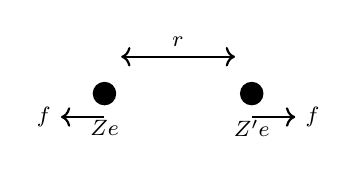
\begin{tikzpicture}[scale=0.85,every node/.style={font=\footnotesize}]
  \fill (-1.1,0) circle (5pt) node[below=6pt]{$Ze$};
  \fill (1.1,0) circle (5pt) node[below=6pt]{$Z'e$};
  \draw[<->,thick] (-0.85,0.55) -- (0.85,0.55) node[midway,above]{$r$};
  \draw[->,thick] (-1.1,-0.35) -- (-1.75,-0.35) node[left]{$f$};
  \draw[->,thick] (1.1,-0.35) -- (1.75,-0.35) node[right]{$f$};
\end{tikzpicture}
\end{center}
\begin{equation}
f = -\frac{k}{r^{2}}\,,\qquad V = -\frac{k}{r}\,,\qquad k = -Z Z' e^{2}.
\end{equation}

\begin{center}
\fbox{\begin{minipage}{0.52\textwidth}
\begin{tabular}{@{}ll@{}}
$E > 0$ & hyperbolic\\
$E = 0$ & parabolic\\
$E < 0$ & elliptic
\end{tabular}\\[4pt]
Only for $V = -\dfrac{k}{r}$ !!!
\end{minipage}}
\end{center}

Scattering requires unbound trajectories, $E>0$:
\begin{equation}
\frac{1}{r} = C\bigl[\,1 + \varepsilon\cos(\tilde\theta - \tilde\theta\,')\,\bigr],
\qquad
C = \frac{mk}{\ell^{2}} = -\frac{m}{\ell^{2}}\,Z Z' e^{2}.
\label{eq:coulomb-orbit}
\end{equation}

\begin{gather}
\text{Eccentricity}\quad
\varepsilon = \left[1 + \frac{2E\ell^{2}}{m k^{2}}\right]^{1/2}
 = \left[1 + \frac{2E\ell^{2}}{m\,(Z Z' e^{2})^{2}}\right]^{1/2}
 = \left[1 + \left(\frac{2sE}{Z Z' e^{2}}\right)^{2}\right]^{1/2} > 1,\\[4pt]
\ell = s\,m\,v_{0} = s\sqrt{2mE}
 \;\longrightarrow\;
 \frac{2\ell^{2}E}{m} = \frac{s^{2}\,2^{2}\,\cancel{m}\,E^{2}}{\cancel{m}}
 = (2sE)^{2}.
\end{gather}

Two situations:
\begin{enumerate}[label=\roman*)]
\item Repulsive case \quad $Z Z' > 0 \;\Rightarrow\; k = -Z Z' e^{2} < 0$;
\item Attractive case \quad $Z Z' < 0 \;\Rightarrow\; k = -Z Z' e^{2} > 0$
      \quad (also gravity, $k = G m_{1} m_{2}$).
\end{enumerate}

\subsection{Repulsive Case: \texorpdfstring{$k<0$}{k<0}, \texorpdfstring{$C=mk/\ell^2<0$}{C=mk/l2<0}}

\begin{align}
\frac{1}{r} = C\bigl[1 + \varepsilon\cos(\tilde\theta-\tilde\theta\,')\bigr] > 0
&\iff 1 + \varepsilon\cos(\tilde\theta-\tilde\theta\,') < 0\notag\\
&\iff \varepsilon\cos(\tilde\theta-\tilde\theta\,') < -1
 \iff \cos(\tilde\theta-\tilde\theta\,') < -\frac{1}{\varepsilon}.
\end{align}

We need the cosine to be \underline{negative} and larger in magnitude than
$1/\varepsilon$. In this case $\tilde\theta = \tilde\theta\,'$ is not a physical
point, because
\begin{equation}
\cos(\tilde\theta\,'-\tilde\theta\,') = \cos(0) = 1
\;\Longrightarrow\;
\underbrace{\frac{1}{r} = C\,[1+\varepsilon] < 0}_{\text{unphysical}}\,.
\end{equation}

So $\tilde\theta = \tilde\theta\,'$ lies in the middle of the inaccessible
region of the hyperbola, and $\tilde\theta = \tilde\theta\,' \pm \pi$ is the
periapsis; we choose $\tilde\theta\,' = \pi$, giving
\begin{equation}
\cos(\tilde\theta - \tilde\theta\,') = \cos(\tilde\theta - \pi)
 = \cos\tilde\theta\,\underbrace{\cos\pi}_{-1}
 + \sin\tilde\theta\,\underbrace{\sin\pi}_{0}
 = -\cos\tilde\theta.
\end{equation}

\begin{equation}
\frac{1}{r} = \left(-\frac{mk}{\ell^{2}}\right)
   \bigl[-1 - \varepsilon\cos(\tilde\theta-\tilde\theta\,')\bigr]
 = \frac{m Z Z' e^{2}}{\ell^{2}}\bigl[\varepsilon\cos\tilde\theta - 1\bigr],
\qquad
\begin{aligned}
&\text{maximum at } \tilde\theta = 0 \;\Rightarrow\\
&\text{minimum } r:\ \frac{1}{r_{m}} = \frac{m Z Z' e^{2}}{\ell^{2}}\,[\varepsilon-1].
\end{aligned}
\end{equation}

So the angle at the apsidal point is $\tilde\theta = 0$. We now need
\begin{equation}
\psi = \tilde\theta(r\to\infty) = \tilde\theta\!\left(\tfrac{1}{r}\to 0\right),
\qquad
\left[\ \text{repulsive case: } \theta = \pi - 2\psi
 \;\Rightarrow\; \psi = \frac{\pi-\theta}{2}\ \right]
\end{equation}
\begin{equation}
0 = \varepsilon\cos\psi - 1
\iff \frac{1}{\varepsilon} = \cos\psi = \cos\!\left(\frac{\pi-\theta}{2}\right)
 = \underbrace{\cos\half{\pi}}_{0}\cos\half{\theta}
 + \underbrace{\sin\half{\pi}}_{1}\sin\half{\theta}
 = \sin\frac{\theta}{2}\,.
\label{eq:rep-sinhalf}
\end{equation}

\subsection{Attractive Case: \texorpdfstring{$k>0$}{k>0}, \texorpdfstring{$C=km/\ell^2>0$}{C=km/l2>0}}

Take $\tilde\theta\,' = 0$:
\begin{equation}
\tilde\theta = \tilde\theta\,' = 0 \;\Rightarrow\;
\frac{1}{r} = C\bigl[1 + \varepsilon\cos(0)\bigr] = C\,[1+\varepsilon],
\qquad
\begin{aligned}
&\text{max at } \tilde\theta = 0\\
&\text{minimum } r:\ \frac{1}{r_{m}} = C\,[1+\varepsilon].
\end{aligned}
\end{equation}

The apsidal point is also at $\tilde\theta = 0$. We now need
\begin{equation}
\psi = \tilde\theta(r\to\infty) = \tilde\theta\!\left(\tfrac{1}{r}\to 0\right),
\qquad
\left[\ \text{attractive case: } \theta = 2\psi - \pi
 \;\Rightarrow\; \psi = \frac{\pi+\theta}{2}\ \right]
\end{equation}
\begin{equation}
0 = 1 + \varepsilon\cos\psi
\iff -\frac{1}{\varepsilon} = \cos\psi = \cos\!\left(\frac{\pi+\theta}{2}\right)
 = \underbrace{\cos\half{\pi}}_{0}\cos\half{\theta}
 - \underbrace{\sin\half{\pi}}_{1}\sin\half{\theta}
 = -\sin\frac{\theta}{2}\,.
\label{eq:att-sinhalf}
\end{equation}

\subsection{Combining Both Cases: the Rutherford Cross Section}

Equations \eqref{eq:rep-sinhalf} and \eqref{eq:att-sinhalf} give the same
relation $1/\varepsilon = \sin(\theta/2)$ in both cases, so
\begin{gather}
\cot^{2}\frac{\theta}{2} = \frac{1}{\tan^{2}\frac{\theta}{2}}
 = \frac{\cos^{2}\frac{\theta}{2}}{\sin^{2}\frac{\theta}{2}}
 = \frac{1-\sin^{2}\frac{\theta}{2}}{\sin^{2}\frac{\theta}{2}}
 = \frac{1}{\sin^{2}\frac{\theta}{2}} - 1
 = \varepsilon^{2} - 1
 = \left(\frac{2sE}{Z Z' e^{2}}\right)^{2}\\[4pt]
\Longrightarrow\qquad
\boxeq{\ s = s(\theta,E) = \left\lvert \frac{Z Z' e^{2}}{2E}\right\rvert
   \cot\frac{\theta}{2}\ }
\label{eq:s-of-theta}
\end{gather}

\begin{align}
\dd{s}{\theta}
 &= \left\lvert \frac{Z Z' e^{2}}{2\varepsilon}\right\rvert
    \dd{}{\theta}\!\left(\frac{\cos\frac{\theta}{2}}{\sin\frac{\theta}{2}}\right)
  = \left\lvert \frac{Z Z' e^{2}}{2\varepsilon}\right\rvert
    \left(\frac{1}{2}\!\left(\frac{-\sin\frac{\theta}{2}}{\sin\frac{\theta}{2}}\right)
      - \frac{1}{2}\,\frac{\cos^{2}\frac{\theta}{2}}{\sin^{2}\frac{\theta}{2}}\right)
  = -\left\lvert \frac{Z Z' e^{2}}{4E}\right\rvert
    \frac{1}{\sin^{2}\frac{\theta}{2}}\,,\footnotemark\\[6pt]
\sigma(\theta)
 &= \frac{s}{\sin\theta}\left\lvert \dd{s}{\theta}\right\rvert
  = \frac{1}{2}\left(\frac{Z Z' e^{2}}{2E}\right)^{\!2}
    \frac{1}{2\sin\frac{\theta}{2}\,\cancel{\cos\frac{\theta}{2}}}\,
    \frac{\cancel{\cos\frac{\theta}{2}}}{\sin\frac{\theta}{2}}\,
    \frac{1}{\sin^{2}\frac{\theta}{2}}\,.
\end{align}
\footnotetext{The first two forms carry $\varepsilon$ in the denominator; the
line switches to $E$ (consistent with Eq.~\eqref{eq:s-of-theta}) in the final
simplification. The inconsistency is retained rather than normalized.}

\begin{equation}
\boxeq{\ \sigma(\theta) = \frac{1}{4}\left(\frac{Z Z' e^{2}}{2E}\right)^{\!2}
  \csc^{4}\!\left(\frac{\theta}{2}\right)\ }
\qquad
\begin{aligned}
&\text{Rutherford scattering cross section}\\
&\text{(for Coulomb forces)}
\end{aligned}
\label{eq:rutherford}
\end{equation}

\noindent\textbf{Remarks:}
\begin{enumerate}[label=\arabic*)]
\item The cross section is the same for the repulsive and attractive cases,
      since it is proportional to $(ZZ')^{2}$.
\item It diverges like $E^{-2}$ at low energies.
\item It diverges like $\theta^{-4}$ (very strongly) for small angles $\theta$.
\item This classical result is exactly the same as the result obtained in
      quantum mechanics.
\end{enumerate}

\section{Total Cross Section}

\begin{equation}
\sigma_{T} = \int \sigma(\Om)\,d\Om ,
\qquad\text{in this case}\quad
\sigma(\theta) = \text{const}\,\frac{1}{\sin^{4}\!\left(\frac{\theta}{2}\right)} .
\end{equation}

\begin{gather}
d\Om = 2\pi\sin\theta\,d\theta = 4\pi\sin\half{\theta}\cos\half{\theta}\,d\theta\\[4pt]
\sigma_{T} = \frac{4\pi}{4}\left(\frac{Z Z' e^{2}}{2E}\right)^{\!2}
  \int_{0}^{\pi}
  \frac{\sin\frac{\theta}{2}\cos\frac{\theta}{2}}{\sin^{4}\frac{\theta}{2}}\,d\theta,
\qquad \text{range: } 0 < \theta \le \pi
\end{gather}
(Fig.~\ref{fig:centre}). Near $\theta = 0$ the integrand behaves as
\begin{equation}
\sim \int_{0}^{\delta}\frac{d\theta}{\left(\frac{\theta}{2}\right)^{3}}
 = 8\int_{0}^{\delta}\frac{d\theta}{\theta^{3}}
 = 8\left.\frac{\theta^{-2}}{(-2)}\right|_{0}^{\,\delta} = +\infty
\qquad \text{strongly divergent}.
\end{equation}

\begin{figure}[htbp]
\centering
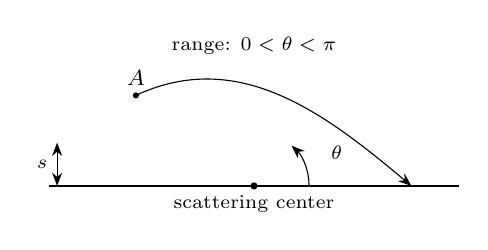
\begin{tikzpicture}[scale=1.0,>=Stealth,every node/.style={font=\footnotesize}]
  \draw[thick] (-2.6,0) -- (2.6,0);
  \coordinate (SC) at (0,0);
  \fill (SC) circle (1.3pt);
  \node[below] at (SC) {\scriptsize scattering center};
  \coordinate (A) at (-1.5,1.15);
  \fill (A) circle (1.1pt);
  \node[above] at (A) {$A$};
  \draw[->] (A) to[out=25,in=140] (2.0,0);
  \draw[->] (0.7,0) arc (0:47:0.7);
  \node at (1.05,0.42) {\scriptsize $\theta$};
  \node[above] at (0,1.55) {\scriptsize range: $0<\theta<\pi$};
  \draw[<->] (-2.5,0.55) -- (-2.5,0) node[midway,left]{\scriptsize $s$};
\end{tikzpicture}
\caption{As $\theta$ ranges over $(0,\pi)$ the impact parameter sweeps its
full accessible range about the scattering center.}
\label{fig:centre}
\end{figure}

\begin{center}
\fbox{\begin{minipage}{0.86\textwidth}
\textsc{Notation:}\\[4pt]
\begin{tabular}{@{}ccccl@{}}
\emph{Goldstein} & & \emph{Others} & &\\[2pt]
$\sigma(\Om)$ & $\longleftrightarrow$ & $\dfrac{d\sigma}{d\Om}$ & \quad &
  differential scattering cross section\\[10pt]
$\sigma_{T}$  & $\longleftrightarrow$ & $\sigma$ & &
  total scattering cross section
\end{tabular}
\end{minipage}}
\end{center}

\begin{center}
\begin{tabular}{@{}l@{\quad}p{0.72\textwidth}@{}}
Classical & $\sigma_{T} = +\infty$ for any long-range potential.\\[3pt]
Quantum   & $\sigma_{T} = +\infty$ for some long-range potentials $V(r)$ that
              do not decay fast enough as $r\to\infty$.
\end{tabular}
\end{center}

\begin{caveat}
In a dense conducting material the Coulomb potential is screened,
\begin{equation}
V = -\frac{k}{r}
\;\longrightarrow\;
V^{\text{screen}}(r) = -\frac{k}{r}\,e^{-r/\lambda},
\end{equation}
the screened Coulomb potential (``Yukawa''). In non-conducting materials
$V^{\text{screen}}(r)$ may take a different form, but it still vanishes much
faster than $1/r$.
\end{caveat}

\end{document}
